% ==============================================================================
% reports/sections/results/06_06_explainability.tex
% ==============================================================================

\section{Phân tích khả năng giải thích}

Để làm rõ hành vi dự đoán bên trong của mô hình trên tập mẫu kiểm định, nhóm áp dụng phương pháp giải thích gia tăng Shapley (\textbf{SHAP TreeExplainer} \cite{lundberg2017unified}) kết hợp với việc trích xuất cấu trúc logic của Cây Quyết Định.

\subsection{Phân tích tầm quan trọng đặc trưng bằng SHAP}
Phân tích SHAP được thực hiện trên 500 mẫu đại diện từ tập kiểm định $\Dval$ đối với mô hình Random Forest theo thời gian có cổng. Bảng \ref{tab:shap_top10} liệt kê 10 đặc trưng có giá trị đóng góp trung bình tuyệt đối ($\text{Mean } |\text{SHAP}|$) lớn nhất.

% ==============================================================================
% reports/tables/generated/tab_shap_top10.tex
% ==============================================================================
\begin{table}[htbp]
\centering
\caption{Top 10 đặc trưng mạng có mức độ đóng góp phân loại lớn nhất theo SHAP TreeExplainer trên tập Validation.}
\label{tab:shap_top10}
\resizebox{\textwidth}{!}{%
\begin{tabular}{rlrl}
\toprule
\textbf{Hạng} & \textbf{Tên đặc trưng mạng} & \textbf{Mean $|$SHAP$|$} & \textbf{Ý nghĩa giao thức / thống kê mạng} \\
\midrule
1 & \texttt{Destination Port} & \SHAPTopOneVal & Cổng đích dịch vụ (Port 21 FTP, Port 22 SSH) \\
2 & \texttt{Fwd Packet Length Std} & \SHAPTopTwoVal & Độ lệch chuẩn kích thước gói tin hướng đi (Fwd) \\
3 & \texttt{Avg Fwd Segment Size} & 0.0292 & Kích thước phân đoạn trung bình hướng đi \\
4 & \texttt{Max Packet Length} & 0.0289 & Độ dài gói tin lớn nhất quan sát được trong flow \\
5 & \texttt{Packet Length Mean} & 0.0275 & Độ dài gói tin trung bình của toàn flow \\
6 & \texttt{min\_seg\_size\_forward} & 0.0272 & Kích thước header TCP tối thiểu phía forward \\
7 & \texttt{Packet Length Std} & 0.0271 & Độ lệch chuẩn độ dài toàn bộ gói tin trong flow \\
8 & \texttt{Fwd Packet Length Mean} & 0.0271 & Độ dài gói tin trung bình hướng đi (Fwd) \\
9 & \texttt{Average Packet Size} & 0.0262 & Kích thước gói tin trung bình tổng thể \\
10 & \texttt{Packet Length Variance} & 0.0208 & Phương sai phân bố độ dài gói tin trong flow \\
\bottomrule
\end{tabular}%
}
\end{table}


Kết quả định lượng cho thấy:
\begin{itemize}
    \item Đặc trưng \textbf{\texttt{Destination Port}} có giá trị lớn nhất với $\text{Mean } |\text{SHAP}| = \textbf{\SHAPTopOneVal}$.
    \item Đặc trưng xếp thứ hai là \texttt{Fwd Packet Length Std} đạt giá trị \textbf{\SHAPTopTwoVal}.
    \item Tỷ số đóng góp giữa đặc trưng số 1 và số 2 là xấp xỉ \textbf{\SHAPRatioTopOneTwo\ lần}.
\end{itemize}

Kết quả phân tích SHAP cho thấy mô hình phụ thuộc mạnh vào \texttt{Destination Port} trong kịch bản có cổng được phân tích, tận dụng cổng dịch vụ như một lối tắt phân loại quan trọng giữa lưu lượng bình thường và lưu lượng tấn công FTP (Cổng 21), như được minh họa trực quan trên biểu đồ phân bố giá trị SHAP (Hình \ref{fig:shap_summary}).

\begin{figure}[htbp]
\centering
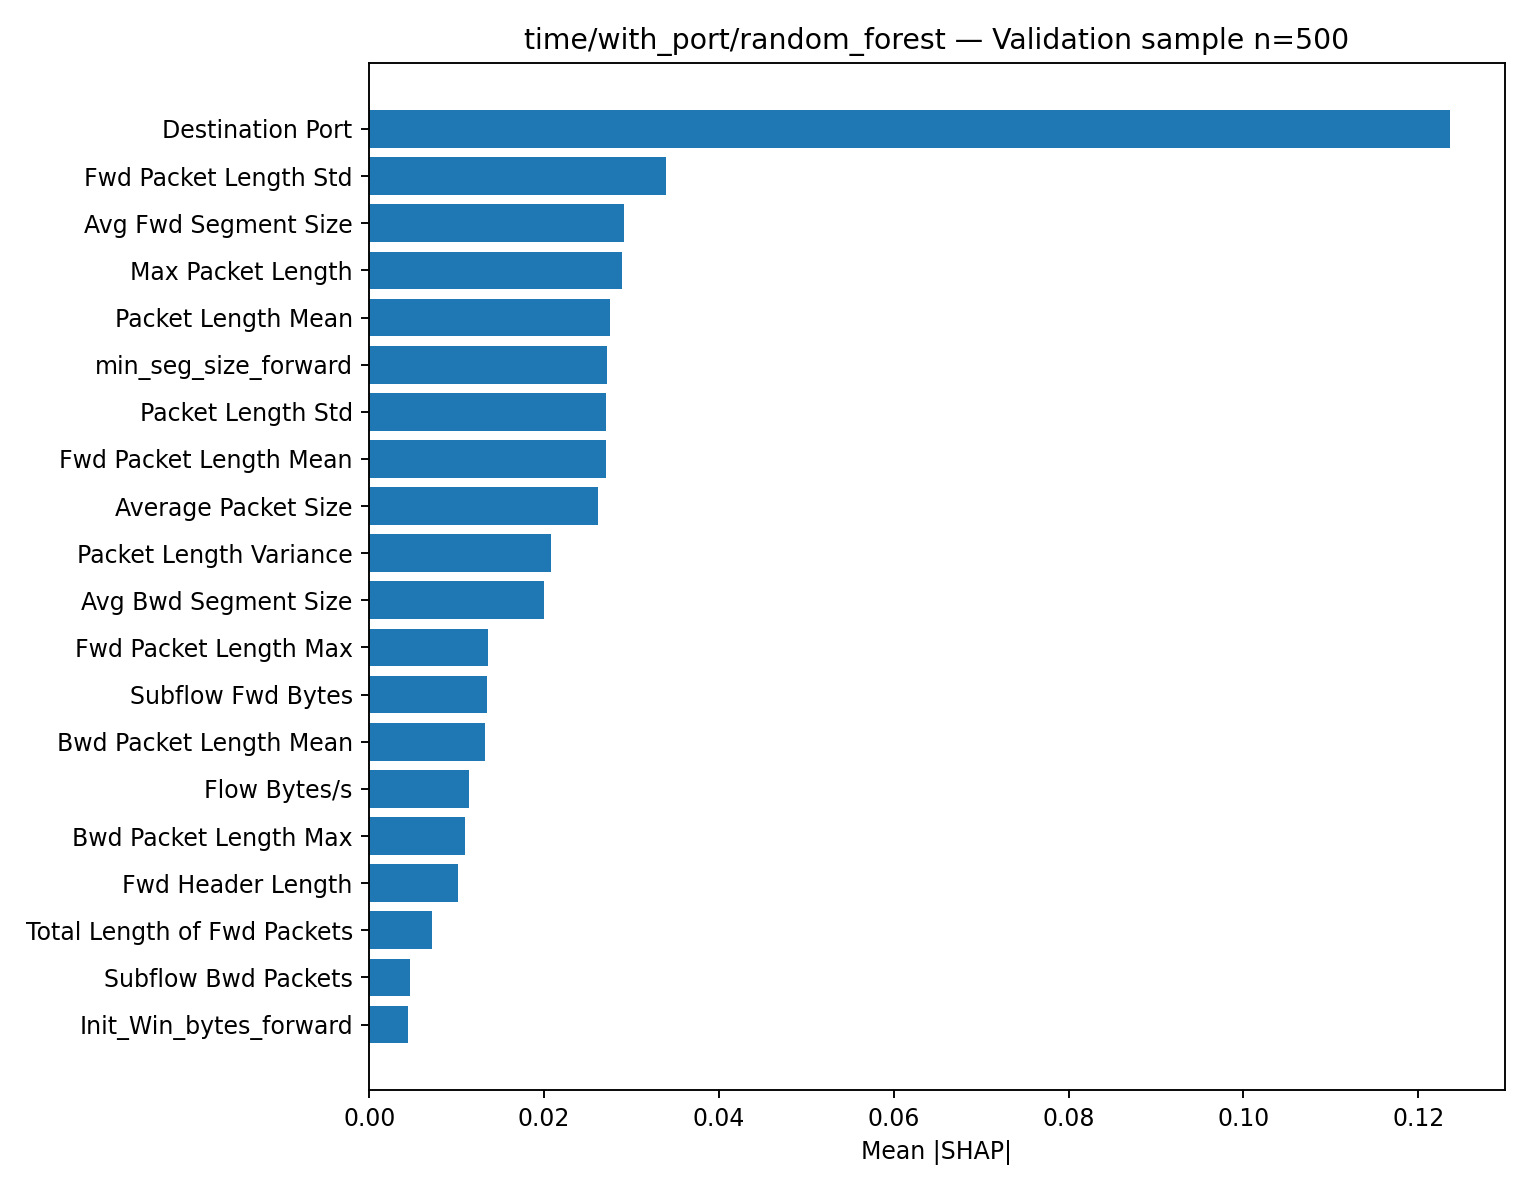
\includegraphics[width=0.85\textwidth]{artifacts/week3_week4/shap/summary.png}
\caption{Biểu đồ phân bố giá trị SHAP (SHAP Summary Plot) của Top các đặc trưng quan trọng trên 500 mẫu kiểm định.}
\label{fig:shap_summary}
\end{figure}

\subsection{Trích xuất cấu trúc cây quyết định}
\label{sec:tree_structure_analysis}
Quan sát cấu trúc logic của Cây Quyết Định càng làm sáng tỏ cơ chế phân nhánh này:
\begin{itemize}
    \item \textbf{Kịch bản có cổng:} Nút gốc (Root Node) phân chia dựa trên điều kiện \texttt{Destination Port <= 21.5} (Hình \ref{fig:tree_structure}). Các nhánh tiếp theo tiếp tục cô lập các flow có \texttt{Destination Port <= 20.5} (loại bỏ traffic cổng thấp) để định vị chính xác \textbf{Cổng 21 (FTP)}.
    \item \textbf{Kịch bản không có cổng:} Khi đặc trưng cổng bị loại bỏ, cây quyết định chọn nút gốc là \texttt{Average Packet Size <= 14.12} (chi tiết quy tắc văn bản trình bày tại Phụ lục \ref{app:tree_rules}).
\end{itemize}

\begin{figure}[htbp]
\centering
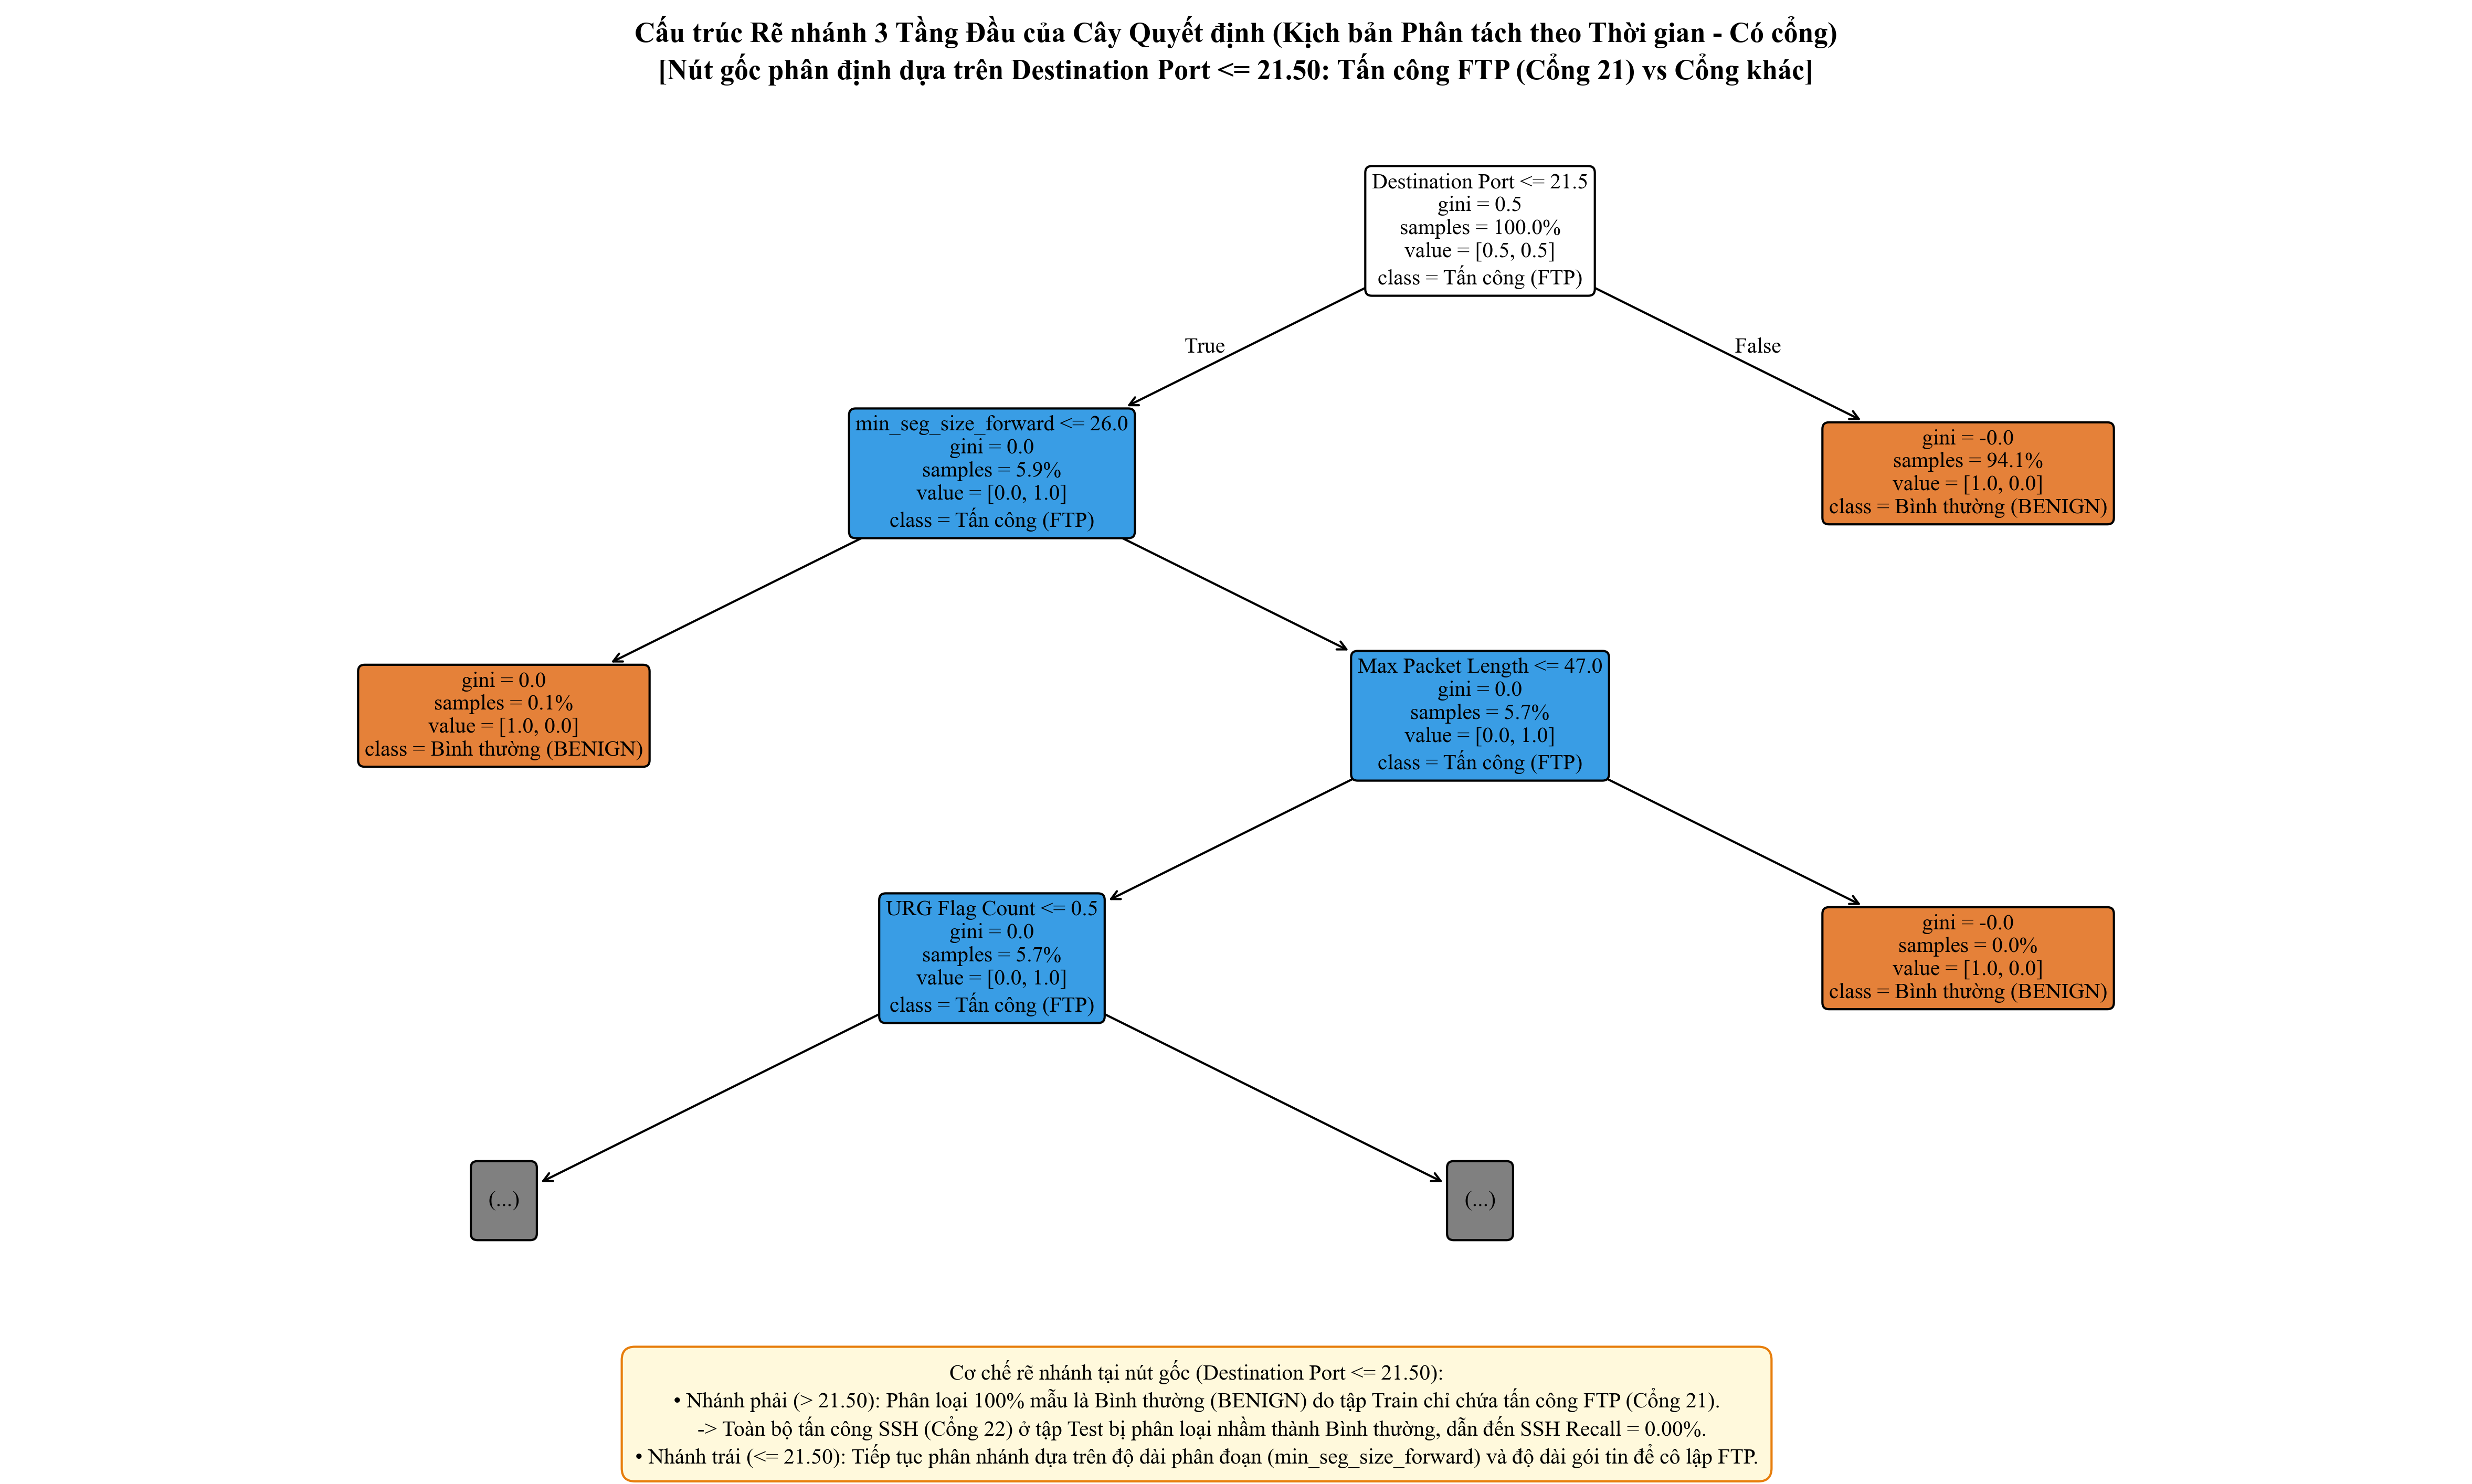
\includegraphics[width=0.95\textwidth]{experiments/figures/01_tree_structure_detailed.png}
\caption{Cấu trúc 3 tầng đầu tiên của Cây Quyết Định minh họa ngưỡng rẽ nhánh ưu tiên tại \texttt{Destination Port $\le$ 21.5}.}
\label{fig:tree_structure}
\end{figure}

Khi chuyển sang tập kiểm thử $\Dtest$, toàn bộ các cuộc tấn công đều diễn ra trên \textbf{Cổng 22 (SSH)}, tức là rơi vào nhánh \texttt{Destination Port > 21.5}. Tại nhánh này, vì trong tập Train mô hình chưa từng thấy cuộc tấn công nào diễn ra trên cổng $> 21$, phần lớn các nút lá tương ứng đều được gán nhãn là lưu lượng bình thường (\Normal, 0). Cấu trúc nhánh rẽ này giải thích vì sao cây quyết định không phát hiện được các flow SSH ở Cổng 22 trong kịch bản có cổng. Cần nhấn mạnh rằng SHAP và cấu trúc cây giải thích hành vi phân loại của mô hình trên tập mẫu quan sát, chứ không chứng minh quan hệ nhân quả trong môi trường mạng thực tế.
